%%%%%%%%%%%%%%%%%%%%%%%%%%%%%%% beamer %%%%%%%%%%%%%%%%%%%%%%%%%%%%%%%%%%%%%%%%%%%%%%%%%
% To run - pdflatex filename.tex
%      acroread filename.pdf
%%%%%%%%%%%%%%%%%%%%%%%%%%%%%%%%%%%%%%%%%%%%%%%%%%%%%%%%%%%%%%%%%%%%%%%%%%%%%%%%%%%%%%%%

\documentclass[compress,oilve]{beamer}
\mode<presentation>

\usetheme[]{CambridgeUS}
% other themes: AnnArbor, Antibes, Bergen, Berkeley, Berlin, Boadilla, boxes, CambridgeUS, Copenhagen, Darmstadt, default, Dresden, Frankfurt, Goettingen,
% Hannover, Ilmenau, JuanLesPins, Luebeck, Madrid, Maloe, Marburg, Montpellier, PaloAlto, Pittsburg, Rochester, Singapore, Szeged, classic

\usecolortheme{beaver}
% color themes: albatross, beaver, beetle, crane, default, dolphin,  fly, lily, orchid, rose, seagull, seahorse, sidebartab, whale, wolverine

\usefonttheme{professionalfonts}
% font themes: default, professionalfonts, serif, structurebold, structureitalicserif, structuresmallcapsserif


\hypersetup{pdfpagemode=FullScreen} % makes your presentation go automatically to full screen

% define your own colors:
\definecolor{Red}{rgb}{1,0,0}
\definecolor{Blue}{rgb}{0,0,1}
\definecolor{Green}{rgb}{0,1,0}
\definecolor{magenta}{rgb}{1,0,.6}
\definecolor{lightblue}{rgb}{0,.5,1}
\definecolor{lightpurple}{rgb}{0.8, 0.6, 0.9}
\definecolor{gold}{rgb}{.6,.5,0}
\definecolor{orange}{rgb}{1,0.4,0}
\definecolor{hotpink}{rgb}{1,0,0.5}
\definecolor{newcolor2}{rgb}{.5,.3,.5}
\definecolor{newcolor}{rgb}{0,.3,1}
\definecolor{newcolor3}{rgb}{1,0,.35}
\definecolor{darkgreen1}{rgb}{0, .35, 0}
\definecolor{darkgreen}{rgb}{0, .6, 0}
\definecolor{darkred}{rgb}{.75,0,0}
\definecolor{skyblue}{HTML}{75bbfd}

\definecolor{olive}{cmyk}{0.64,0,0.95,0.4}
\definecolor{purpleish}{cmyk}{0.75,0.75,0,0}

% can also choose different themes for the "inside" and "outside"

% \usepackage{beamerinnertheme_______}
% inner themes include circles, default, inmargin, rectangles, rounded

% \usepackage{beamerouterthemesmoothbars}
% outer themes include default, infolines, miniframes, shadow, sidebar, smoothbars, smoothtree, split, tree


\useoutertheme[subsection=true, height=40pt]{smoothbars}

% to have the same footer on all slides
%\setbeamertemplate{footline}[text line]{STUFF HERE!}
\setbeamertemplate{footline}[text line]{} % makes the footer EMPTY
% include packages
%

%show the page numbers in footnote
%\addtobeamertemplate{navigation symbols}{}{%
%	\usebeamerfont{footline}%
%	\usebeamercolor[fg]{footline}%
%	\hspace{1em}%
%	\insertframenumber/\inserttotalframenumber
%}

\setbeamercolor{footline}{fg=purpleish}
\setbeamerfont{footline}{series=\bfseries}

%add color to current subsection
\setbeamertemplate{section in head/foot}{\hfill\tikz\node[rectangle, fill=darkred, rounded corners=1pt,inner sep=1pt,] {\textcolor{white}{\insertsectionhead}};}
\setbeamertemplate{section in head/foot shaded}{\textcolor{darkred}{\hfill\insertsectionhead}}

% Remove bullet of subsections
\setbeamertemplate{headline}
{%
	\begin{beamercolorbox}{section in head/foot}
		\insertsectionnavigationhorizontal{\textwidth}{}{}
	\end{beamercolorbox}%
}


% modify headlline, specially headline size
\setbeamertemplate{headline}{%
	\leavevmode%
	\hbox{%
		\begin{beamercolorbox}[wd=\paperwidth,ht=3.5ex,dp=1.125ex]{palette quaternary}%
			\insertsectionnavigationhorizontal{\paperwidth}{}{\hskip0pt plus1filll}
		\end{beamercolorbox}%
	}
}

\setbeamertemplate{footline}{%
	\leavevmode%
	\hbox{\begin{beamercolorbox}[wd=.5\paperwidth,ht=2.5ex,dp=1.125ex,leftskip=.3cm plus1fill,rightskip=.3cm]{author in head/foot}%
			\usebeamerfont{author in head/foot}\insertshortauthor ~ \insertshortinstitute
		\end{beamercolorbox}%
		\begin{beamercolorbox}[wd=.5\paperwidth,ht=2.5ex,dp=1.125ex,leftskip=.3cm,rightskip=.3cm plus1fil]{title in head/foot}%
			\usebeamerfont{title in head/foot}\insertshorttitle\hfill\insertframenumber\,/\,\inserttotalframenumber
	\end{beamercolorbox}}%
	\vskip0pt%
}


%\setbeamertemplate{navigation symbols}{}

\title{AutoEncoders}
\author{ML Instruction Team, Fall 2022}
\institute[]{CE Department \newline  Sharif University of Technology \newline \newline}
\date[\today]{}
%\titlegraphic{\includegraphics[scale=.35]{example-image}}



%Write \usepackage{etex} just after the \documentclass line (it should be the first loaded package).
\usepackage{etex}
\usepackage{subcaption}
\usepackage{multicol}
\usepackage{amsmath}
\usepackage{epsfig}
\usepackage{graphicx}
\usepackage[all,knot]{xy}
\xyoption{arc}
\usepackage{url}
\usepackage{multimedia}
\usepackage{hyperref}
\hypersetup{colorlinks,linkcolor=blue,citecolor=redorange,urlcolor=darkred}
\usepackage{multirow}
\usepackage[font={scriptsize}]{caption}
\usepackage{pgf}
\usepackage{fontspec}
%\setsansfont[Scale=MatchLowercase, BoldFont = * Bold, ItalicFont = * Italic]{Caladea}

%\usepackage{enumitem,xcolor}
%\newcommand{\labelitemi}{$\blacksquare$}
%\newcommand{\labelitemii}{$\diamond$}
%\newcommand{\labelitemiii}{$\square$}
%\newcommand{\labelitemiv}{$\ast$}
%\setbeamercolor*{item}{fg=red}


\usefonttheme{professionalfonts} 
\setbeamertemplate{itemize item}{\color{skyblue}$\blacksquare$}
\setbeamertemplate{itemize subitem}{\color{hotpink}$\blacktriangleright$}
\setbeamertemplate{itemize subsubitem}{\color{orange}$\bullet$}


\usepackage{anyfontsize}
\usepackage{t1enc}
\usepackage{tikz}
\usetikzlibrary{calc,trees,positioning,arrows,chains,shapes.geometric,decorations.pathreplacing,decorations.pathmorphing,shapes,matrix,shapes.symbols}



\newtheorem{proposition}[theorem]{Proposition}
\newtheorem{remark}[theorem]{Remark}
\newtheorem{assumption}[theorem]{Assumption}

\usepackage{fontspec,unicode-math}
\setmainfont{Consolas}[
    Scale=0.9,
    Path=./Fonts/,
    Extension = .ttf,
]
\setmonofont{Monaco}[
    Scale=0.9,
    Path=./Fonts/,
    Extension = .ttf,
]

\setsansfont[Scale=1]{Times New Roman}

\graphicspath{{figs/}}

%\usepackage{smartdiagram}
%\usesmartdiagramlibrary{additions}
%%%%%%%%%%%%%%%%%%%%%%%%%%%%%%%%%%%%%%%%%%%%%%%%%%%%%%%%%%%%%%%%%%%%%%%%%%%%%%%%%%%%%%%%%%%%
%%%%%%%%%%%%%%%%%%%%%%%%%%%%%% Title Page Info %%%%%%%%%%%%%%%%%%%%%%%%%%%%%%%%%%%%%%%%%%%
%%%%%%%%%%%%%%%%%%%%%%%%%%%%%%%%%%%%%%%%%%%%%%%%%%%%%%%%%%%%%%%%%%%%%%%%%%%%%%%%%%%%%%%%%%


%%%%%%%%%%%%%%%%%%%%%%%%%%%%%%%%%%%%%%%%%%%%%%%%%%%%%%%%%%%%%%%%%%%%%%%%%%%%%%%%%%%%%%%%%%
%%%%%%%%%%%%%%%%%%%%%%%%%%%%%% Begin Your Document %%%%%%%%%%%%%%%%%%%%%%%%%%%%%%%%%%%%%%%
%%%%%%%%%%%%%%%%%%%%%%%%%%%%%%%%%%%%%%%%%%%%%%%%%%%%%%%%%%%%%%%%%%%%%%%%%%%%%%%%%%%%%%%%%%
\begin{document}
	
%%%%%%%%%%%%%%%%%%%%%%%%%%%%%%%%%%%%%%%%%%%%%%%%%%%%%%%%%%%%%%%%%%%%%%%%%%%%%%%%%%%%%%%%%%
	\fontsize{9}{9}
\begin{frame}[noframenumbering, plain]
	\titlepage
\end{frame}

%%%%%%%%%%%%%%%%%%%%%%%%%%%%%%%%%%%%%%%%%%%%%%%%%%%%%%%%%%%%%%%%%%%%%%%%%%%%%%%%%%%%%%%%%%
\section{Introduction}
%%%%%%%%%%%%%%%%%%%%%%%%%%%%%%%%%%%%%%%%%%%%%%%%%%%%%%%%%%%%%%%%%%%%%%%%######

\frame{\frametitle{Autoencoders}
	
	
\begin{itemize}
	\item 
	Autoencoders are artificial neural networks capable of learning dense representations
    of the input data, called \textit{latent representations} or \textit{codings}, without any supervision (i.e., the training set is unlabeled).

	\item 
	Their job is to take an input $X$ and predict $X$.
	To make this non-trivial, we need to add a {\color{hotpink} bottleneck layer} whose
    dimension is much smaller than the input.

    \hyperlink{ae_arch}{
    \begin{figure}[htp]
    \vspace{1ex}%
    \centering
    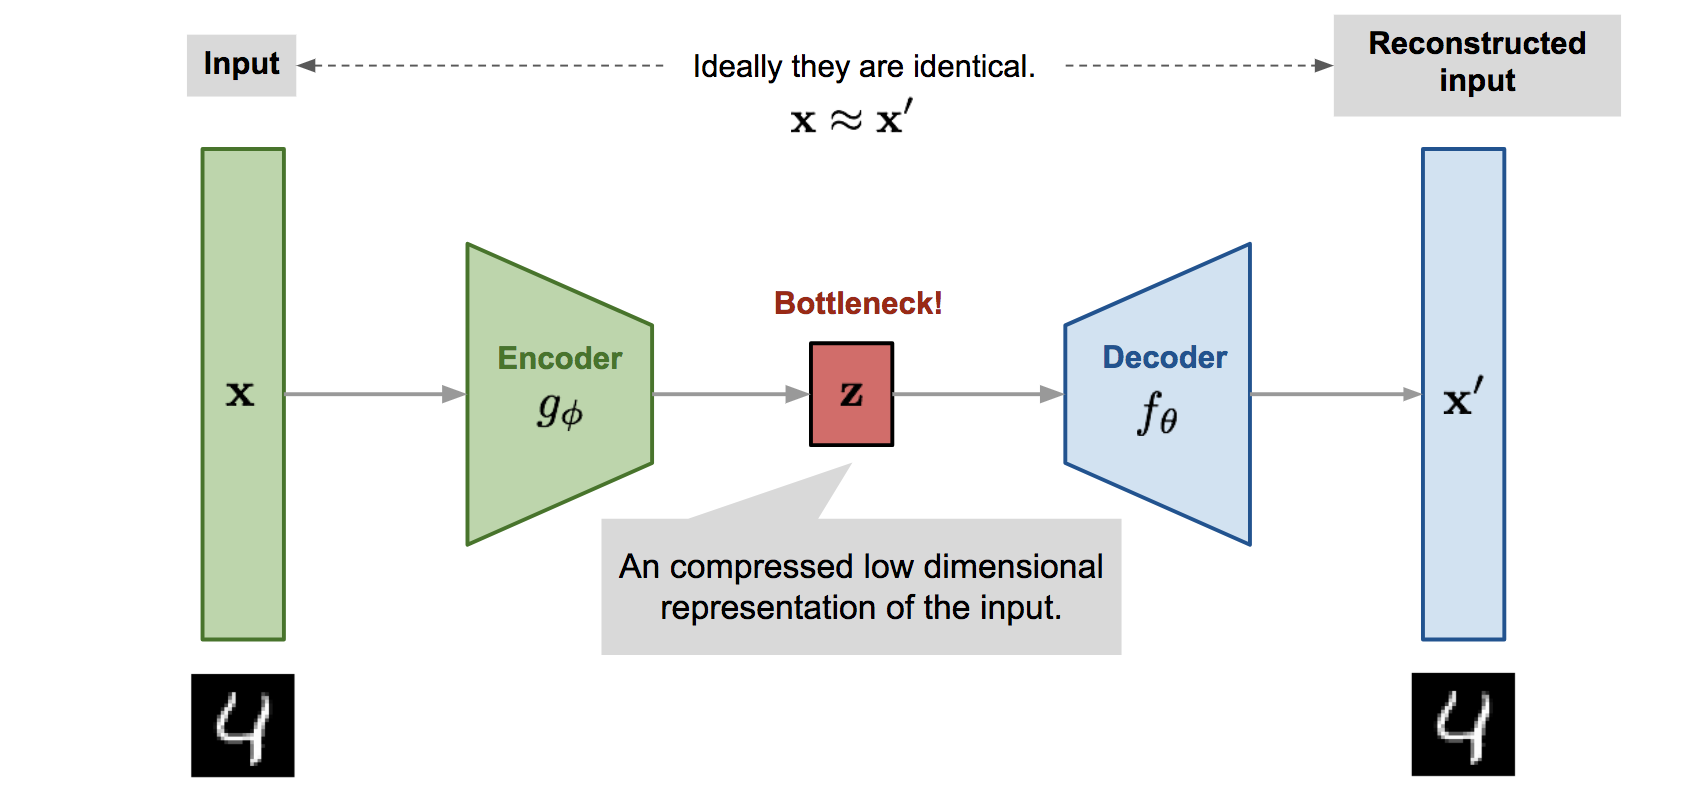
\includegraphics[width=10cm]{autoencoder-architecture}
    \end{figure}}
	
	
\end{itemize}	
	
}

%%%%%%%%%%%%%%%%%%%%%%%%%%%%%%%%%%%%%%%%%%%%%%%%%%%%%%%%%%%%%%%%%%%%%%%%%%%%%%%%%%%%%%%%%%%%%%%
\frame{\frametitle{Autoencoders: Structure}
	
\begin{itemize}
	\item 
	Encoder:  compress input into a latent-space of usually smaller dimension.  $h = f(x)$


	\item 
	Decoder: reconstruct input from the latent space. $r = g(f(x))$ with $r$ as close to $x$ as possible

    \hyperlink{bad_ae}{
    \begin{figure}[htp]
    \vspace{1ex}%
    \centering
    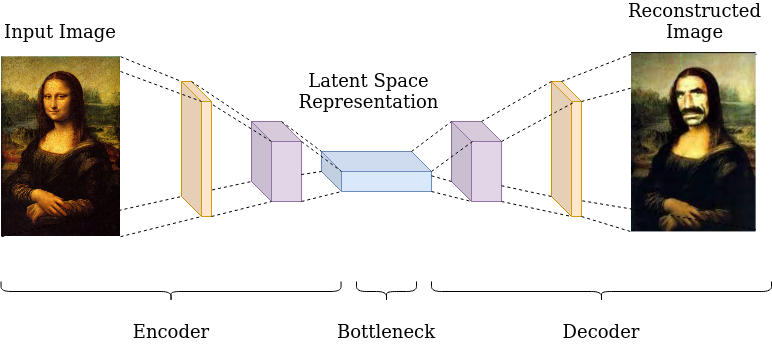
\includegraphics[width=10cm]{Bad_AE}
    \end{figure}}
	
	
\end{itemize}	
	
}

%%%%%%%%%%%%%%%%%%%%%%%%%%%%%%%%%%%%%%%%%%%%%%%%%%%%%%%%%%%%%%%%%%%%%%%%%%%%%%%%%%%%%%%%%%%%%%%

\frame{\frametitle{Autoencoders: Applications}
	
\begin{itemize}
	\item 
	Autoencoders can 
	\begin{itemize}
		\item act as feature detectors
		\item be used for unsupervised pretraining of deep neural networks
	\end{itemize}

    \hyperlink{AE}{
    \begin{figure}[htp]
    \vspace{1ex}%
    \centering
    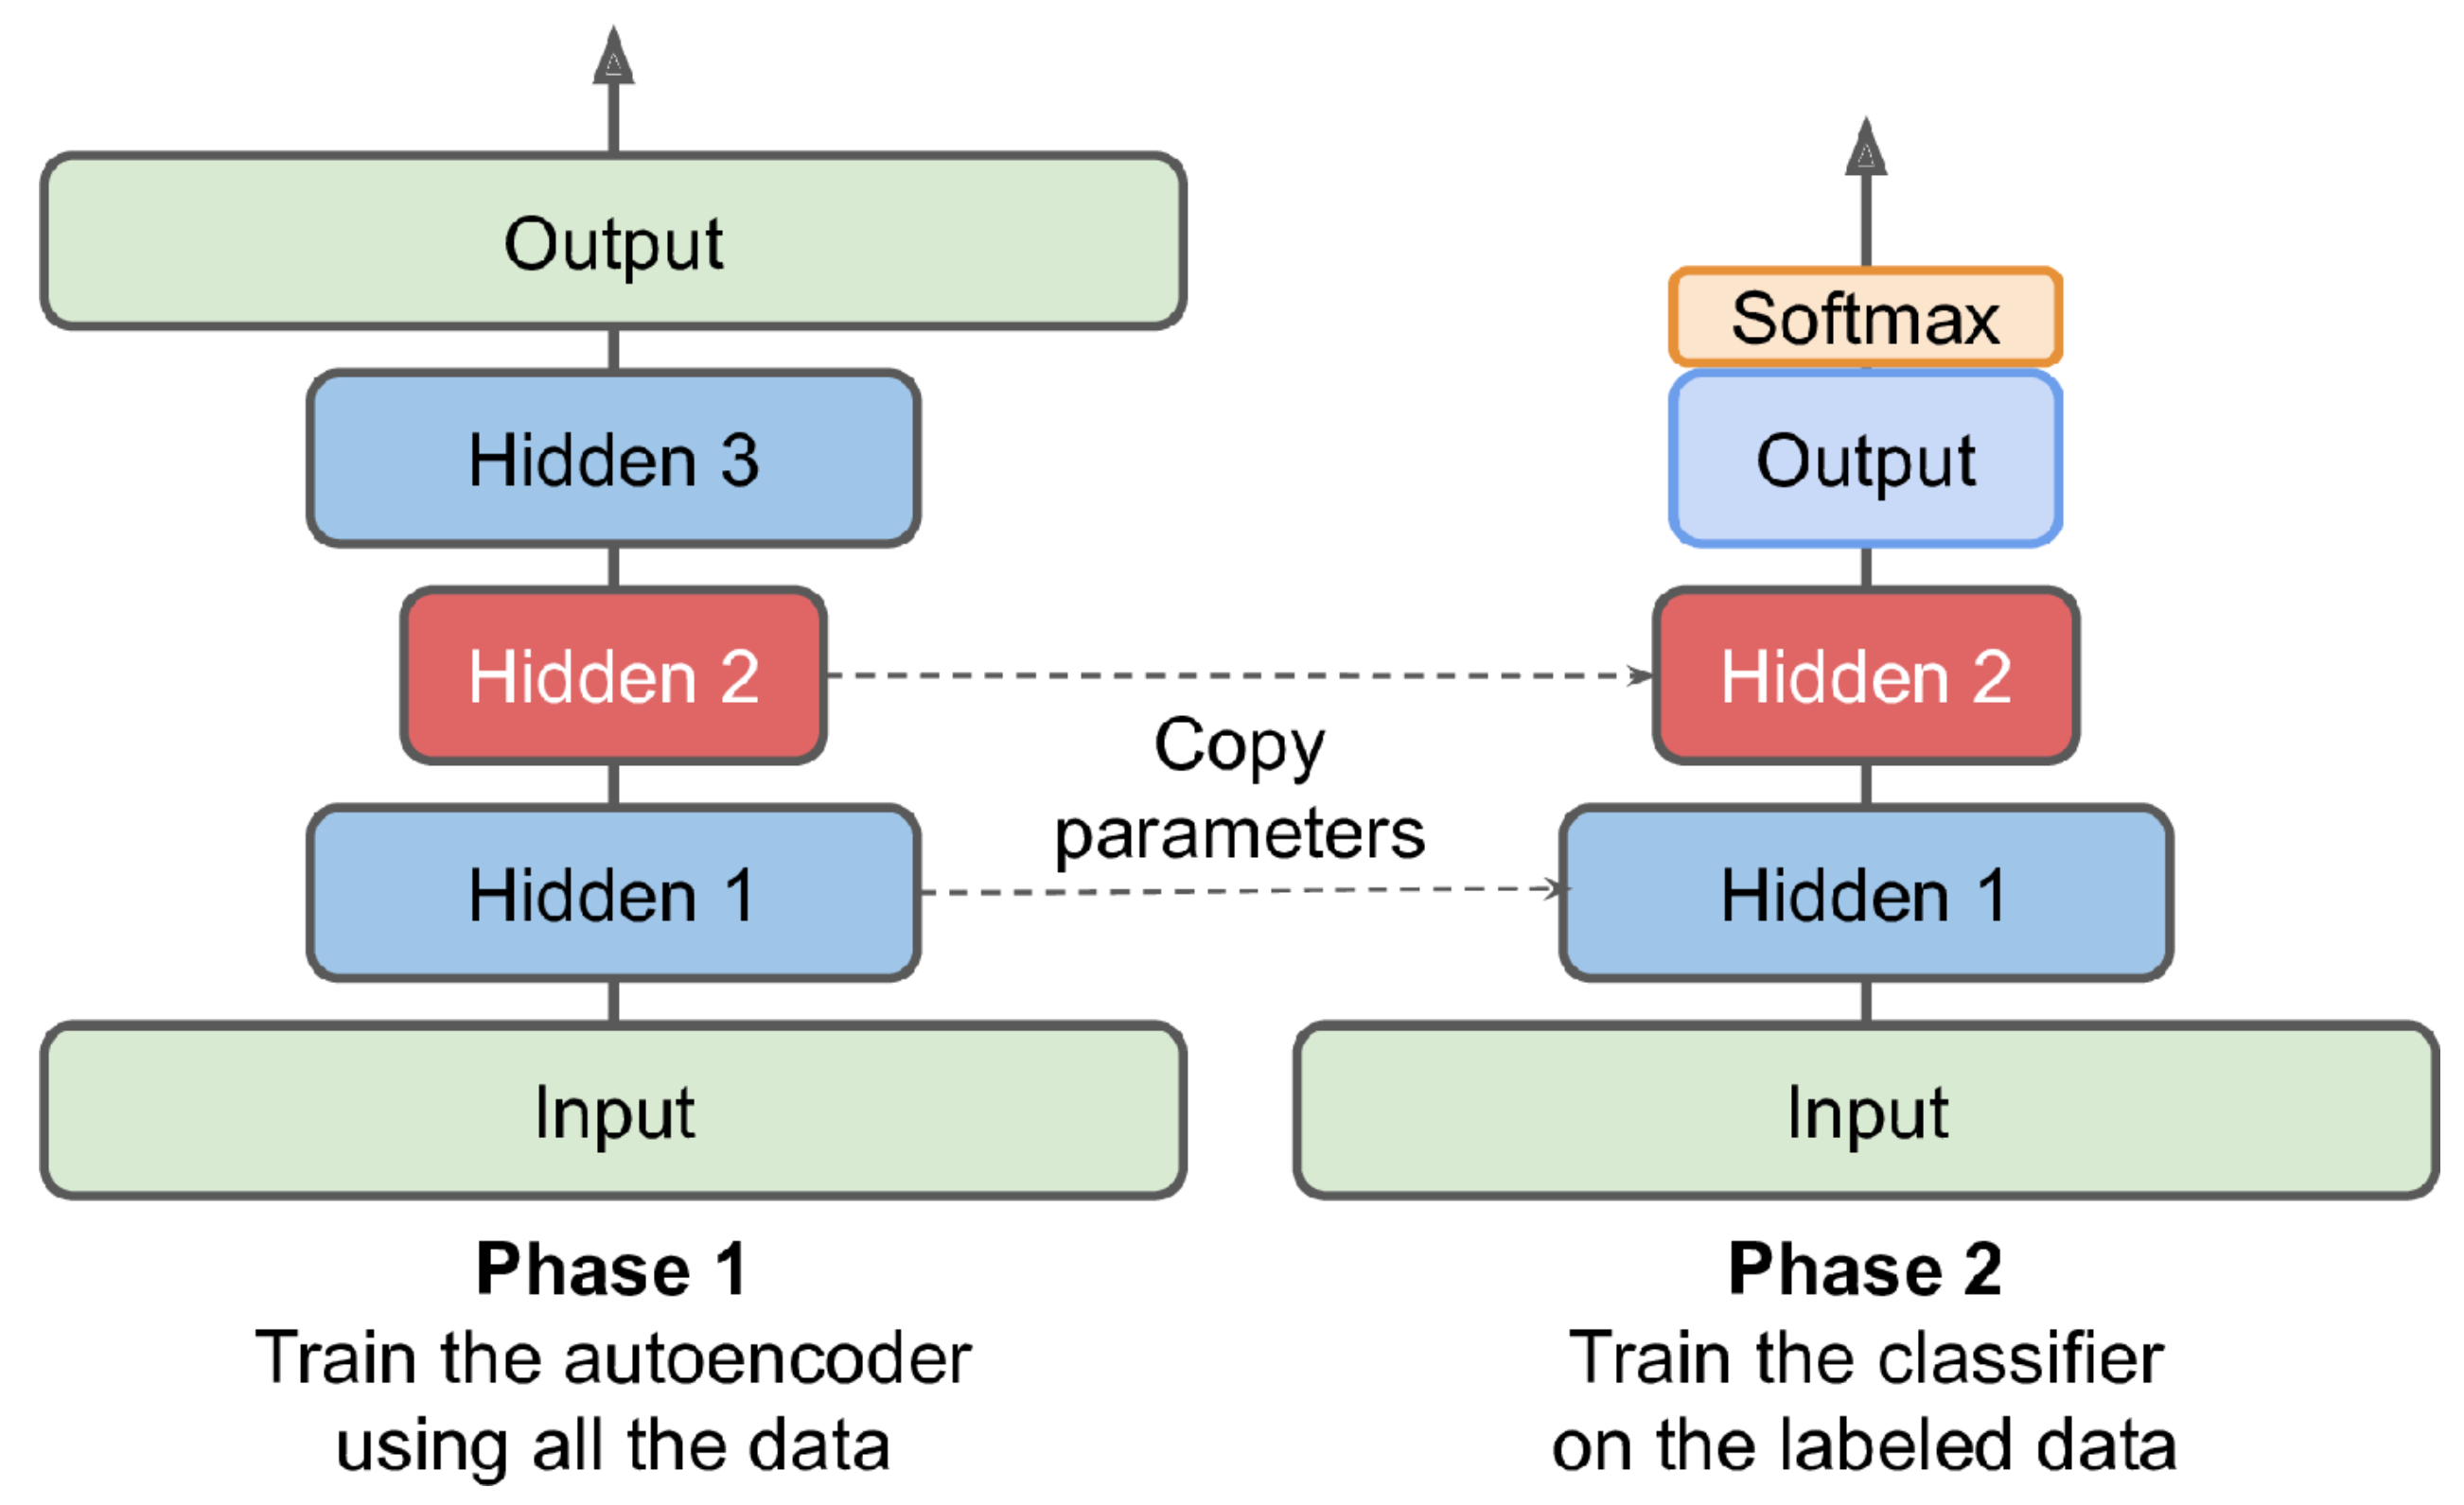
\includegraphics[width=8cm]{AE_application}
    \end{figure}}
	
	
\end{itemize}	
	
}
%%%%%%%%%%%%%%%%%%%%%%%%%%%%%%%%%%%%%%%%%%%%%%%%%%%%%%%%%%%%%%%%%%%%%%%%%%%%%%%%%%%%%%%%%%%%%%%

\frame{\frametitle{Autoencoders: Applications}
	
\begin{itemize}
	\item 
	Autoencoders can be used as generative models. (will be discussed more later in this chapter.) 

    
    \hyperlink{generated_by_VAE}{
    \begin{figure}[htp]
    \vspace{2ex}%
    \centering
    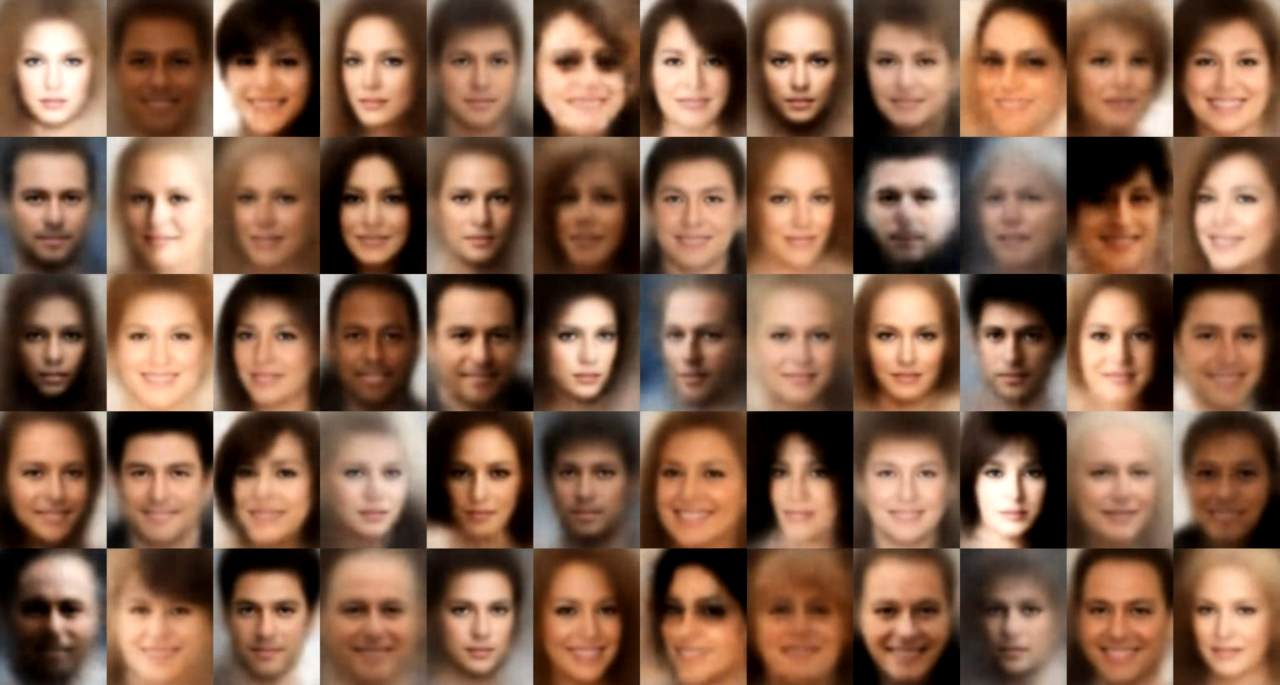
\includegraphics[width=8cm]{generated_by_VAE}
    \end{figure}}
	
	
\end{itemize}	
	
}

%%%%%%%%%%%%%%%%%%%%%%%%%%%%%%%%%%%%%%%%%%%%%%%%%%%%%%%%%%%%%%%%%%%%%%%%%%%%%%%%%%%%%%%%%%%%%%%

\frame{\frametitle{Autoencoders: Applications}
	
\begin{itemize}
	\item 
	Watermark removal

    
    \hyperlink{watermark_removal}{
    \begin{figure}[htp]
    \vspace{4ex}%
    \centering
    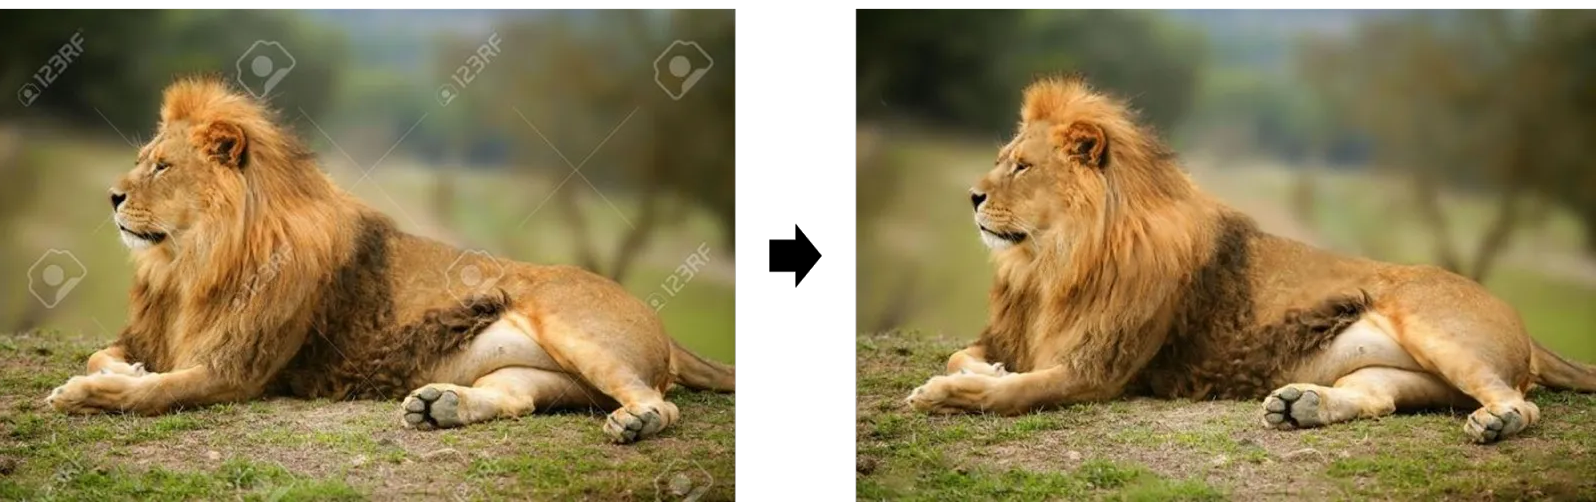
\includegraphics[width=10cm]{watermark_removal}
    \end{figure}}
	
	
\end{itemize}	
	
}

%%%%%%%%%%%%%%%%%%%%%%%%%%%%%%%%%%%%%%%%%%%%%%%%%%%%%%%%%%%%%%%%%%%%%%%%%%%%%%%%%%%%%%%%%%%%%%%

\frame{\frametitle{Autoencoders: Applications}
	
\begin{itemize}
	\item 
	Noise reduction

    
    \hyperlink{noise_reduction}{
    \begin{figure}[htp]
    \vspace{2ex}%
    \centering
    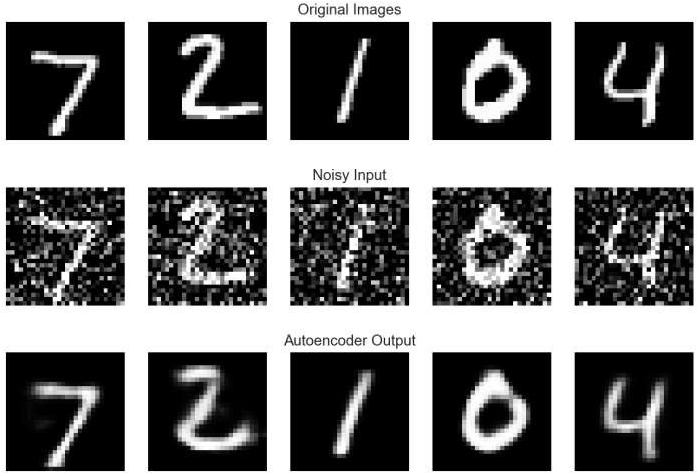
\includegraphics[width=8cm]{noise_reduction}
    \end{figure}}
	
	
\end{itemize}	
	
}

%%%%%%%%%%%%%%%%%%%%%%%%%%%%%%%%%%%%%%%%%%%%%%%%%%%%%%%%%%%%%%%%%%%%%%%%%%%%%%%%%%%%%%%%%%%%%%%

\frame{\frametitle{Stacked Autoencoders}
	
\begin{itemize}
	\item 
	Autoencoders can have multiple hidden layers. In this case they are called \textit{stacked autoencoders} (or \textit{deep autoencoders}).
	\item
	Adding more layers helps the autoencoder learn more complex codings. but be careful about {\color{red}overfitting}!

    

    \hyperlink{stacked_ae}{
    \begin{figure}[htp]
    \vspace{2ex}%
    \centering
    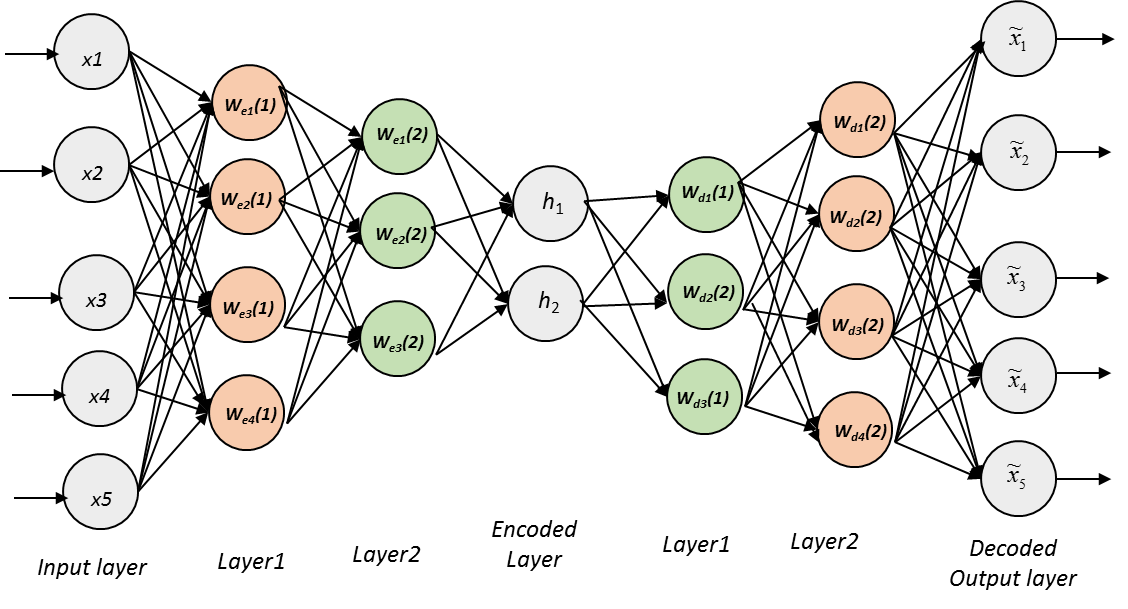
\includegraphics[width=8cm]{stacked_AE}
    \end{figure}}
	
	
\end{itemize}	
	
}

%%%%%%%%%%%%%%%%%%%%%%%%%%%%%%%%%%%%%%%%%%%%%%%%%%%%%%%%%%%%%%%%%%%%%%%%%%%%%%%%%%%%%%%%%%%%%%%

\frame{\frametitle{Autoencoders \& Images}

	
	\centering
    \vspace{30 pt}
    \textbf{\large{Are normal Autoencoders suitable for working with images?}}

    

    \hyperlink{ae_1}{
    \begin{figure}[htp]
    \vspace{2ex}%
    \centering
    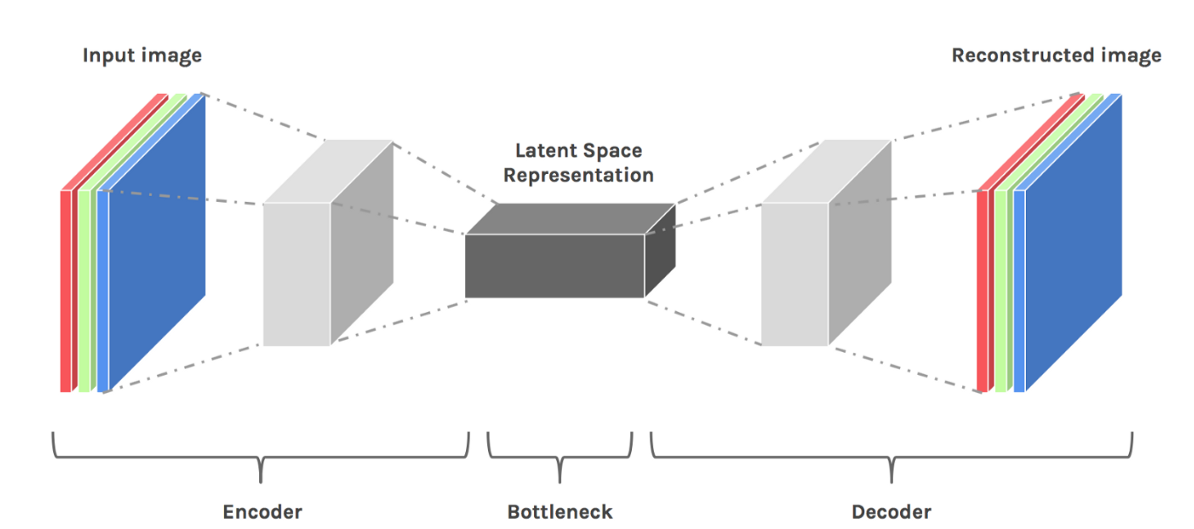
\includegraphics[width=10cm]{AE}
    \end{figure}}
}

%%%%%%%%%%%%%%%%%%%%%%%%%%%%%%%%%%%%%%%%%%%%%%%%%%%%%%%%%%%%%%%%%%%%%%%%%%%%%%%%%%%%%%%%%%%%%%%

\frame{\frametitle{Autoencoders \& Images}

\begin{itemize}	
    \item 
    Convolutional Autoencoders

    

    \hyperlink{cnn_ae}{
    \begin{figure}[htp]
    \vspace{2ex}%
    \centering
    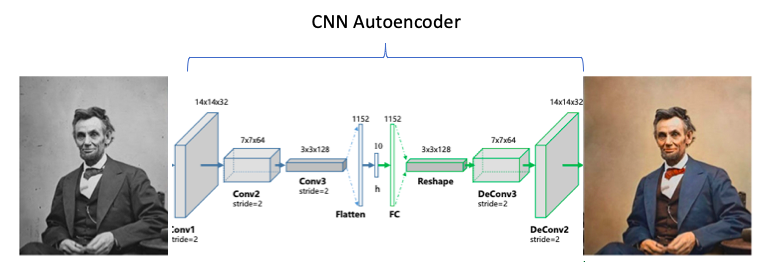
\includegraphics[width=10cm]{cnn_autoencoder}
    \end{figure}}

\end{itemize}
}

%%%%%%%%%%%%%%%%%%%%%%%%%%%%%%%%%%%%%%%%%%%%%%%%%%%%%%%%%%%%%%%%%%%%%%%%%%%%%%%%%%%%%%%%%%%%%%%

\frame{\frametitle{Denoising Autoencoders}

\begin{itemize}	
    \item 
    Another way to force the autoencoder to learn useful features is to add noise to its inputs.
    
    \item 
    Denoising autoencoders train to minimize the loss between $x$ and $g(f(x+w))$, where $w$ is random noise.
    
    \item 
    Denoising autoencoders, with Gaussian noise (left) or dropout (right):


    \hyperlink{AE}{
    \begin{figure}[htp]
    \vspace{1ex}%
    \centering
    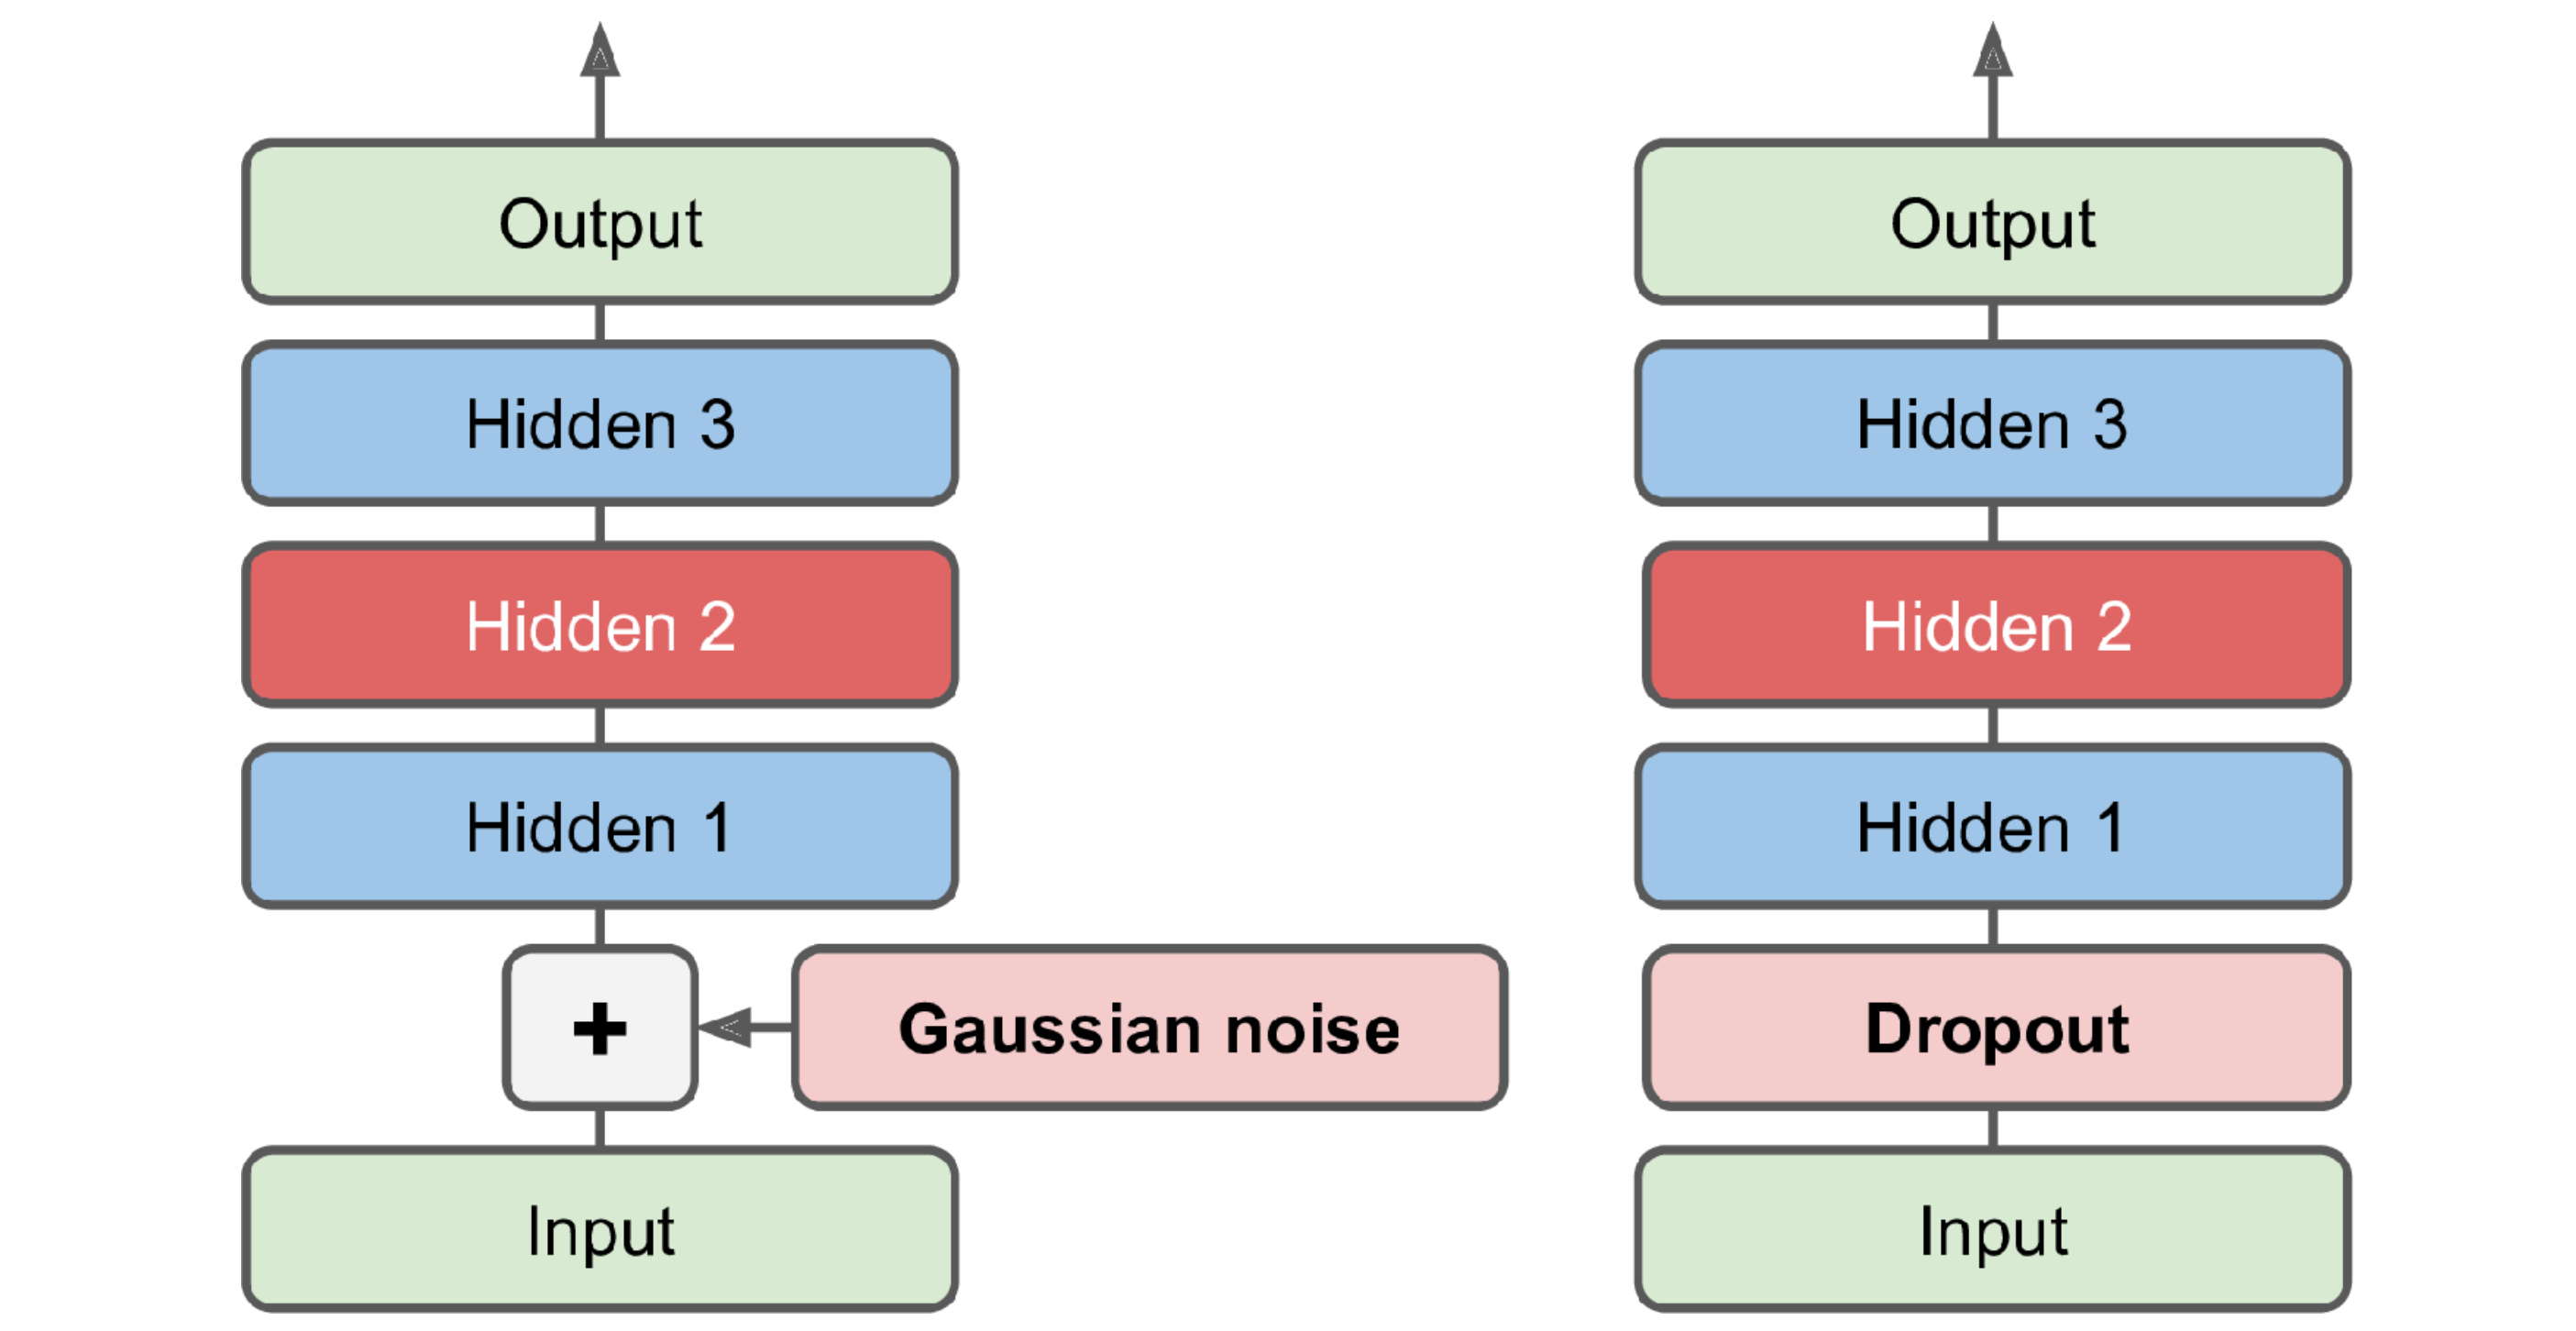
\includegraphics[width=10cm]{denoising_autoencoders}
    \end{figure}}

\end{itemize}
}

%%%%%%%%%%%%%%%%%%%%%%%%%%%%%%%%%%%%%%%%%%%%%%%%%%%%%%%%%%%%%%%%%%%%%%%%%%%%%%%%%%%%%%%%%%%%%%%

\frame{\frametitle{Denoising Autoencoders}

\begin{itemize}	
    \item 
    A few noisy images (with half the pixels turned off), and the images reconstructed by the dropout-based denoising autoencoder. Notice how the autoencoder guesses details that are actually not in the input, such as the top of the white shirt (bottom row, fourth image).

    \hyperlink{AE}{
    \begin{figure}[htp]
    \vspace{1ex}%
    \centering
    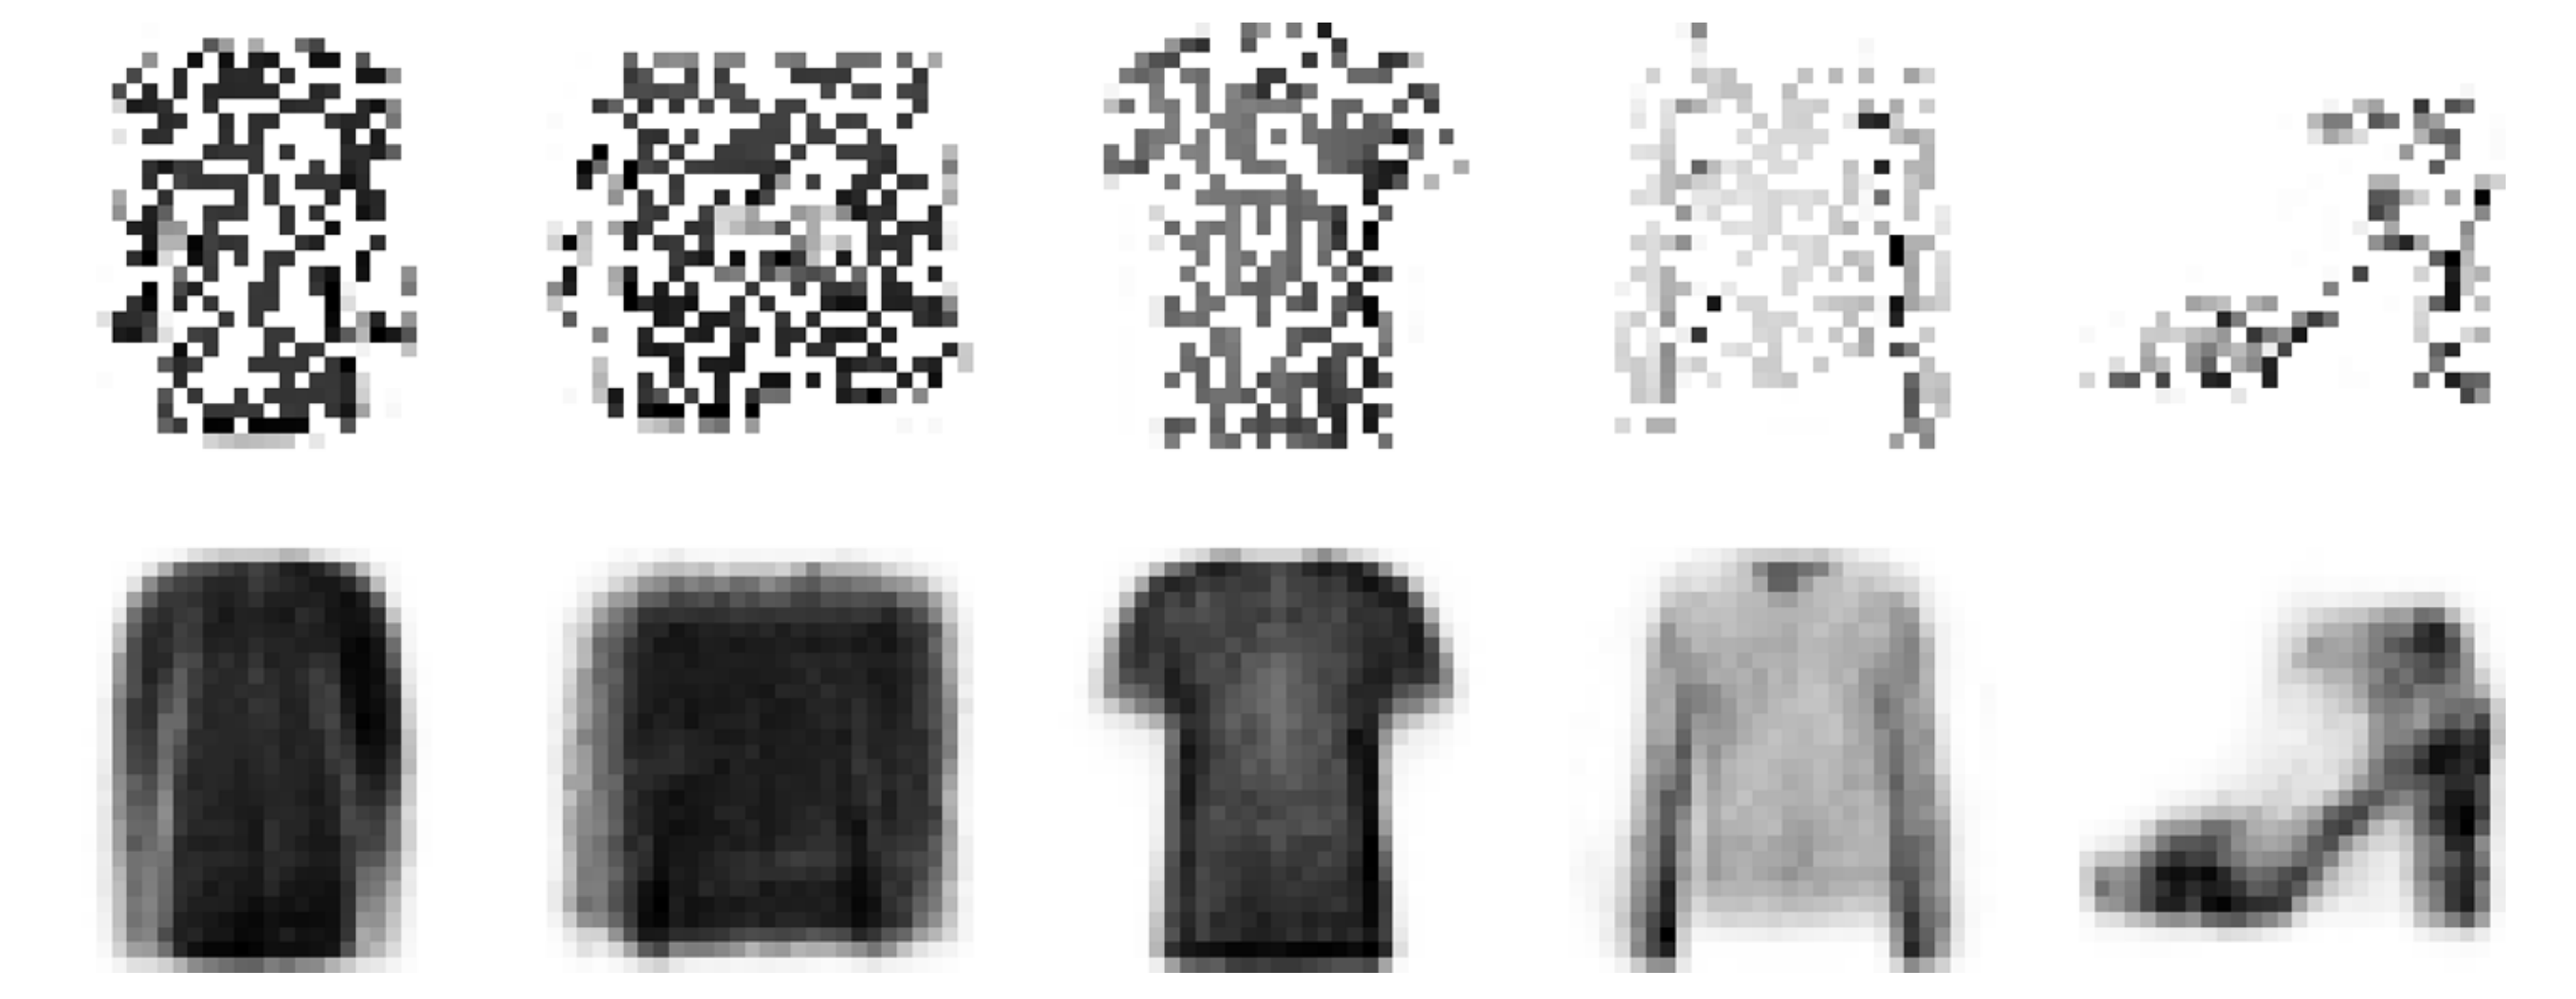
\includegraphics[width=10cm]{denoising_pics}
    \end{figure}}

\end{itemize}
}

%%%%%%%%%%%%%%%%%%%%%%%%%%%%%%%%%%%%%%%%%%%%%%%%%%%%%%%%%%%%%%%%%%%%%%%%%%%%%%%%%%%%%%%%%%%%%%%

\frame{\frametitle{Denoising Autoencoders}

\begin{itemize}	
    \item 
    Intuitively, a denoising autoencoder learns a projection from a neighborhood of our training data back onto the training data.

    \hyperlink{denoising}{
    \begin{figure}[htp]
    \vspace{1ex}%
    \centering
    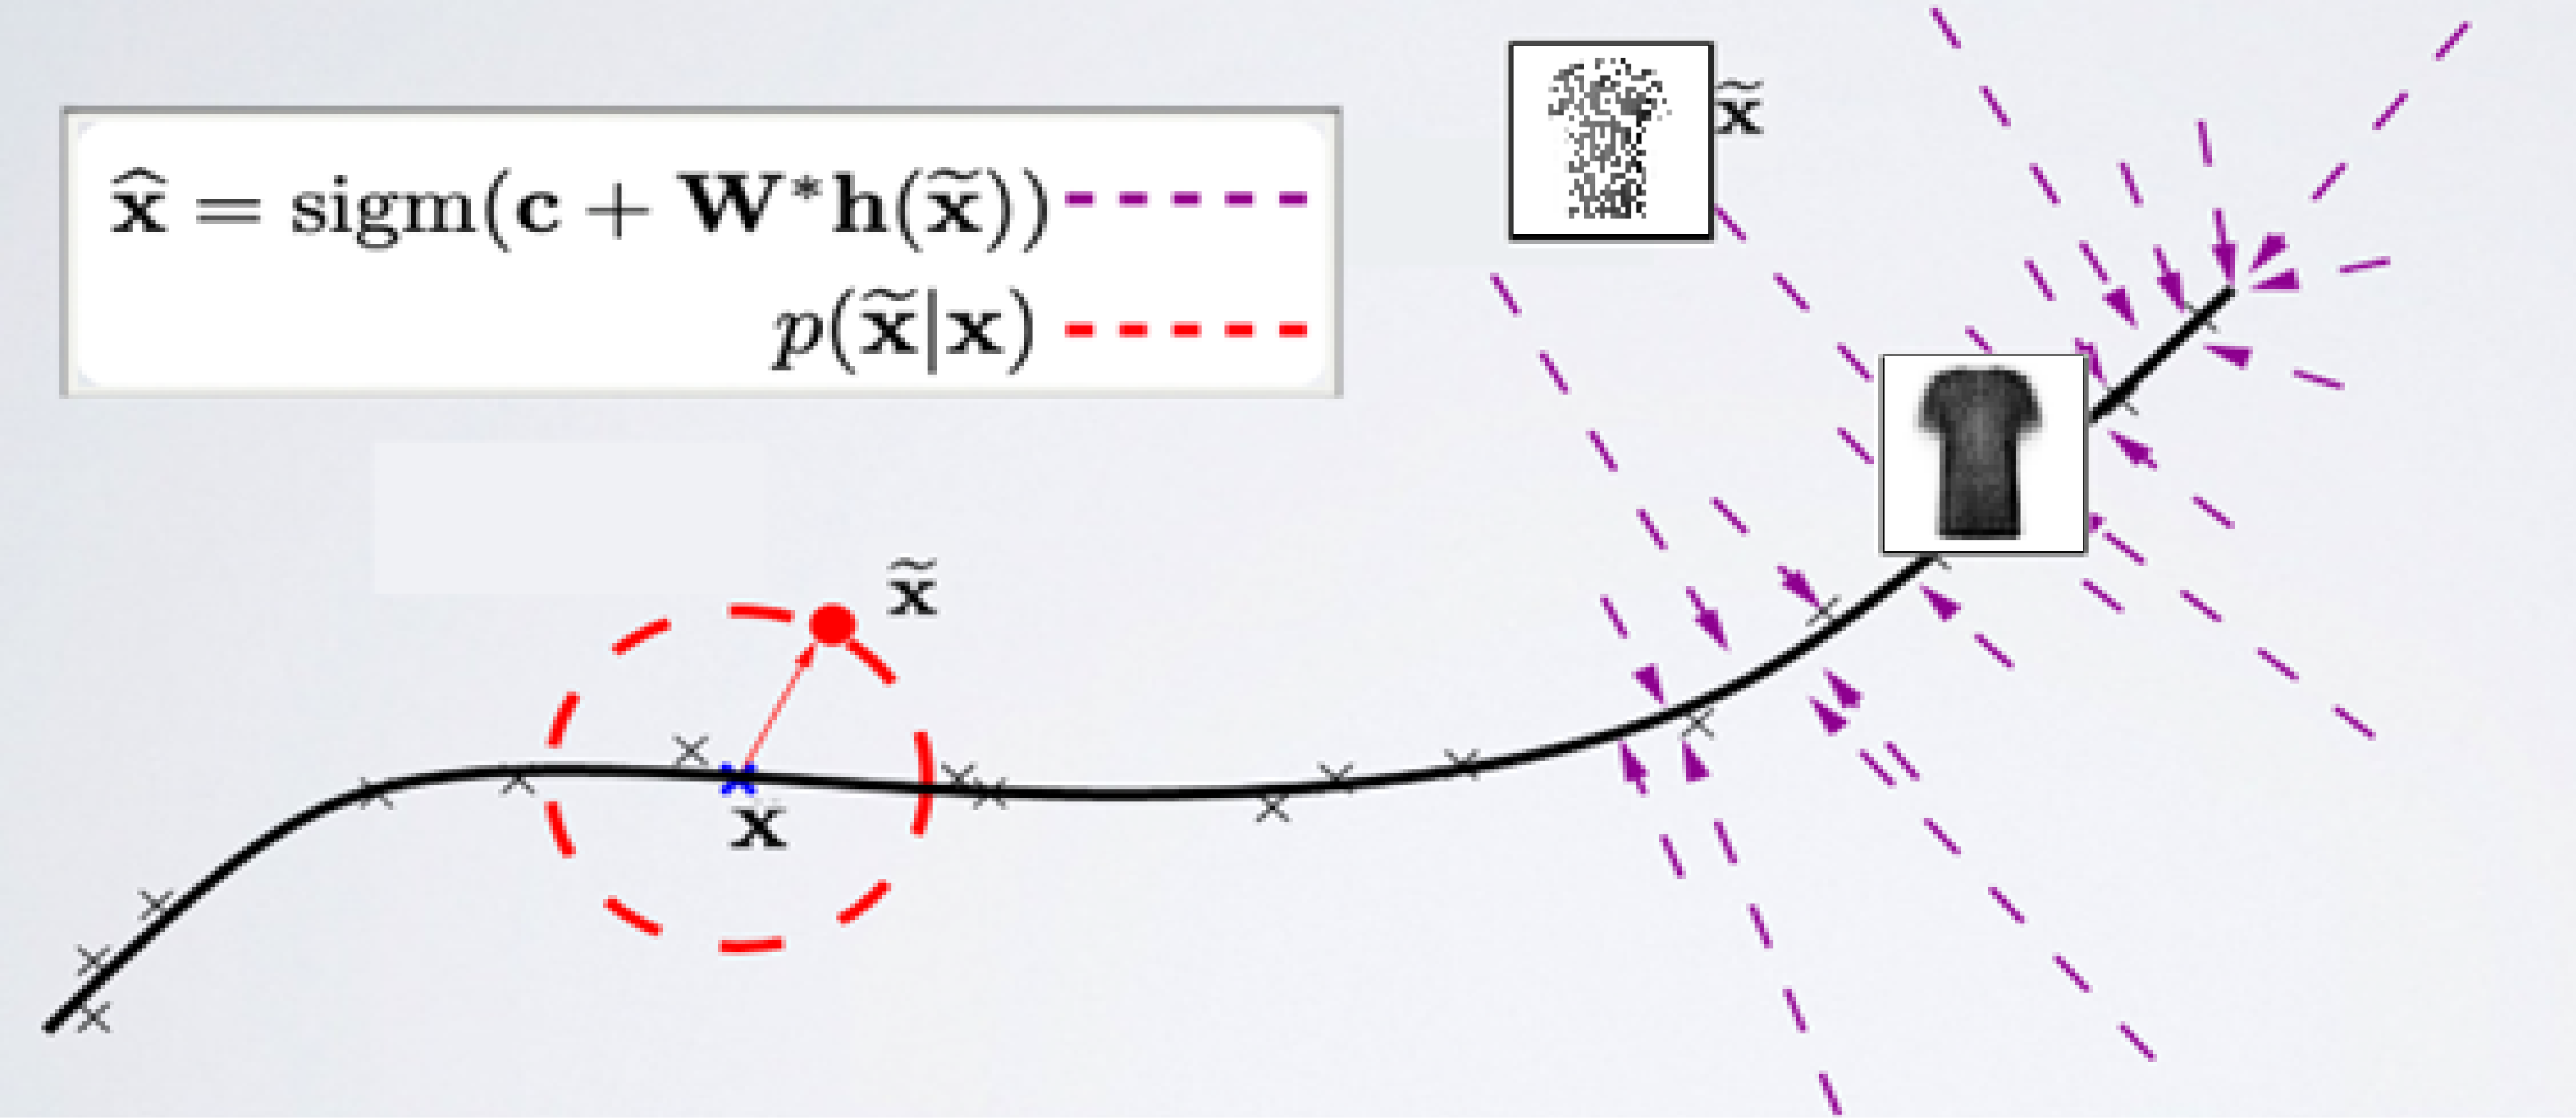
\includegraphics[width=10cm]{denoising}
    \end{figure}}

\end{itemize}
}

%%%%%%%%%%%%%%%%%%%%%%%%%%%%%%%%%%%%%%%%%%%%%%%%%%%%%%%%%%%%%%%%%%%%%%%%%%%%%%%%%%%%%%%%%%%%%%%

\frame{\frametitle{Autoencoder Generative Models}

	
	\centering
    \vspace{25 pt}
    \textbf{\large{How can we generate {\color{hotpink}{NEW}} data with Autoencoders??}}
    \vspace{5 pt}
    \newline
    hint: Autoencoder learns the feature space!

    

}

%%%%%%%%%%%%%%%%%%%%%%%%%%%%%%%%%%%%%%%%%%%%%%%%%%%%%%%%%%%%%%%%%%%%%%%%%%%%%%%%%%%%%%%%%%%%%%%

\frame{\frametitle{Walking through an example}

\begin{itemize}	
    \item 
    We want to reconstruct some shapes.

    \hyperlink{vae}{
    \begin{figure}[htp]
    \vspace{1ex}%
    \centering
    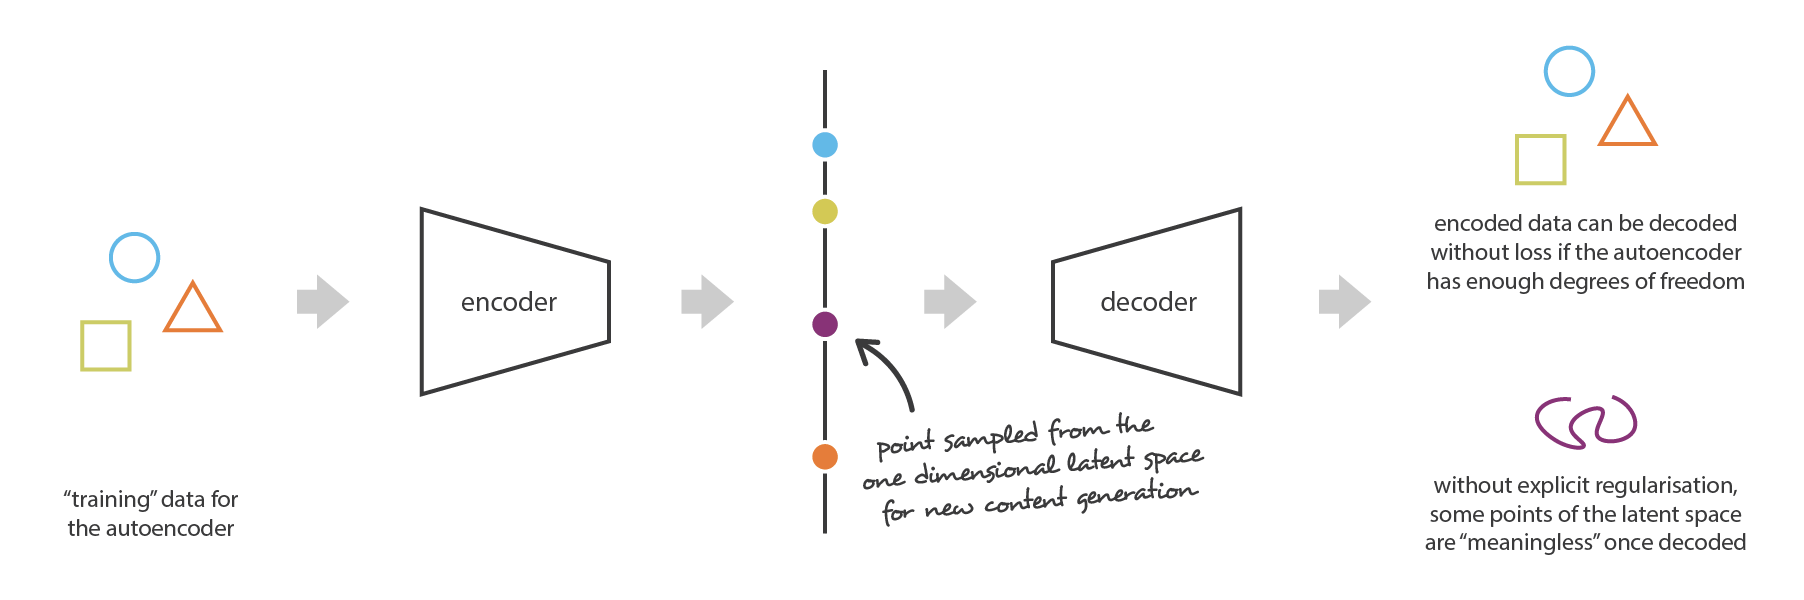
\includegraphics[width=10cm]{vae_1}
    \end{figure}}

\end{itemize}
}

%%%%%%%%%%%%%%%%%%%%%%%%%%%%%%%%%%%%%%%%%%%%%%%%%%%%%%%%%%%%%%%%%%%%%%%%%%%%%%%%%%%%%%%%%%%%%%%

\frame{\frametitle{Walking through an example}

\begin{itemize}	
    \item 
    Not all of the points in latent space have meaningful reconstructions.

    \hyperlink{vae}{
    \begin{figure}[htp]
    \vspace{1ex}%
    \centering
    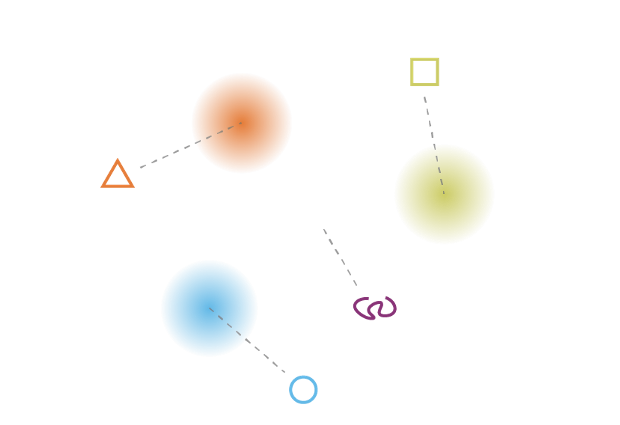
\includegraphics[width=9cm]{vae_2_1}
    \end{figure}}

\end{itemize}
}

%%%%%%%%%%%%%%%%%%%%%%%%%%%%%%%%%%%%%%%%%%%%%%%%%%%%%%%%%%%%%%%%%%%%%%%%%%%%%%%%%%%%%%%%%%%%%%%

\frame{\frametitle{Walking through an example}

\begin{itemize}	
    \item 
    What we want is something like the following picture. So that with sampling from the latent space, we can generate new shapes.

    \hyperlink{vae}{
    \begin{figure}[htp]
    \vspace{1ex}%
    \centering
    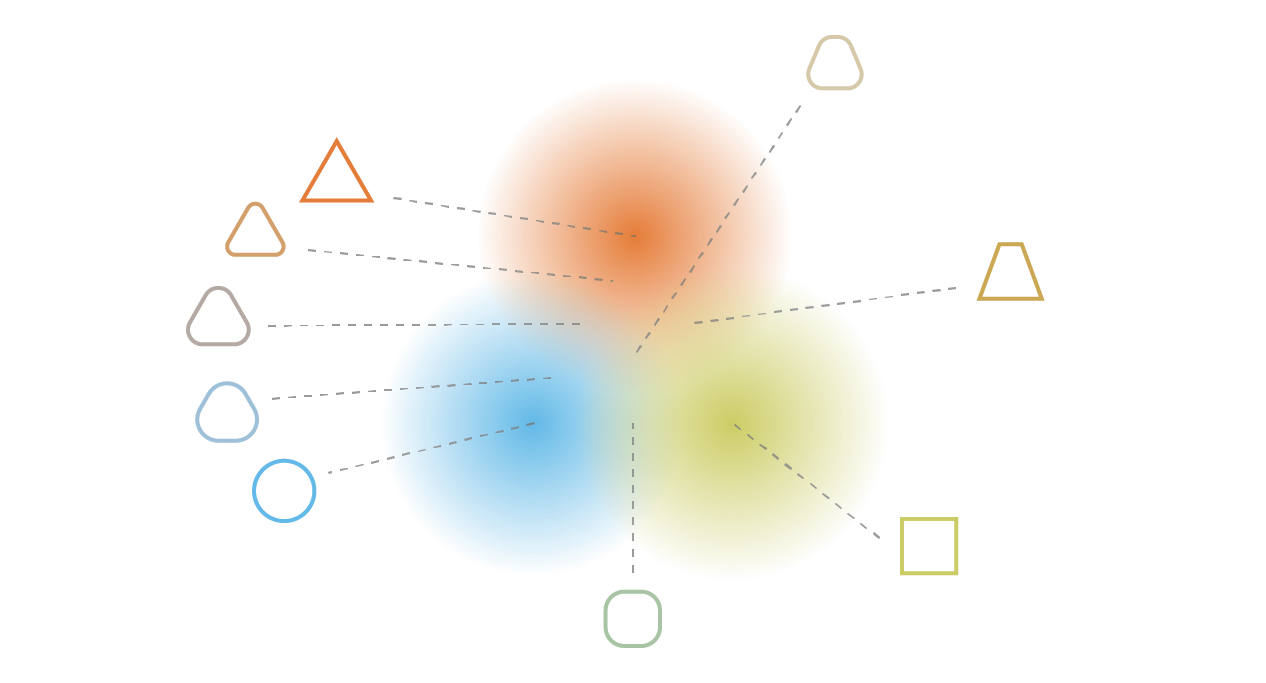
\includegraphics[width=9cm]{vae_3}
    \end{figure}}

\end{itemize}
}

%%%%%%%%%%%%%%%%%%%%%%%%%%%%%%%%%%%%%%%%%%%%%%%%%%%%%%%%%%%%%%%%%%%%%%%%%%%%%%%%%%%%%%%%%%%%%%%

\frame{\frametitle{Variational Autoencoders}

\begin{itemize}	
    \item 
    instead of directly producing a coding for a given input, the encoder produces a mean coding μ and a standard deviation σ. The actual coding is then sampled randomly from a Gaussian distribution with mean μ and standard deviation σ

    \hyperlink{ae}{
    \begin{figure}[htp]
    \vspace{1ex}%
    \centering
    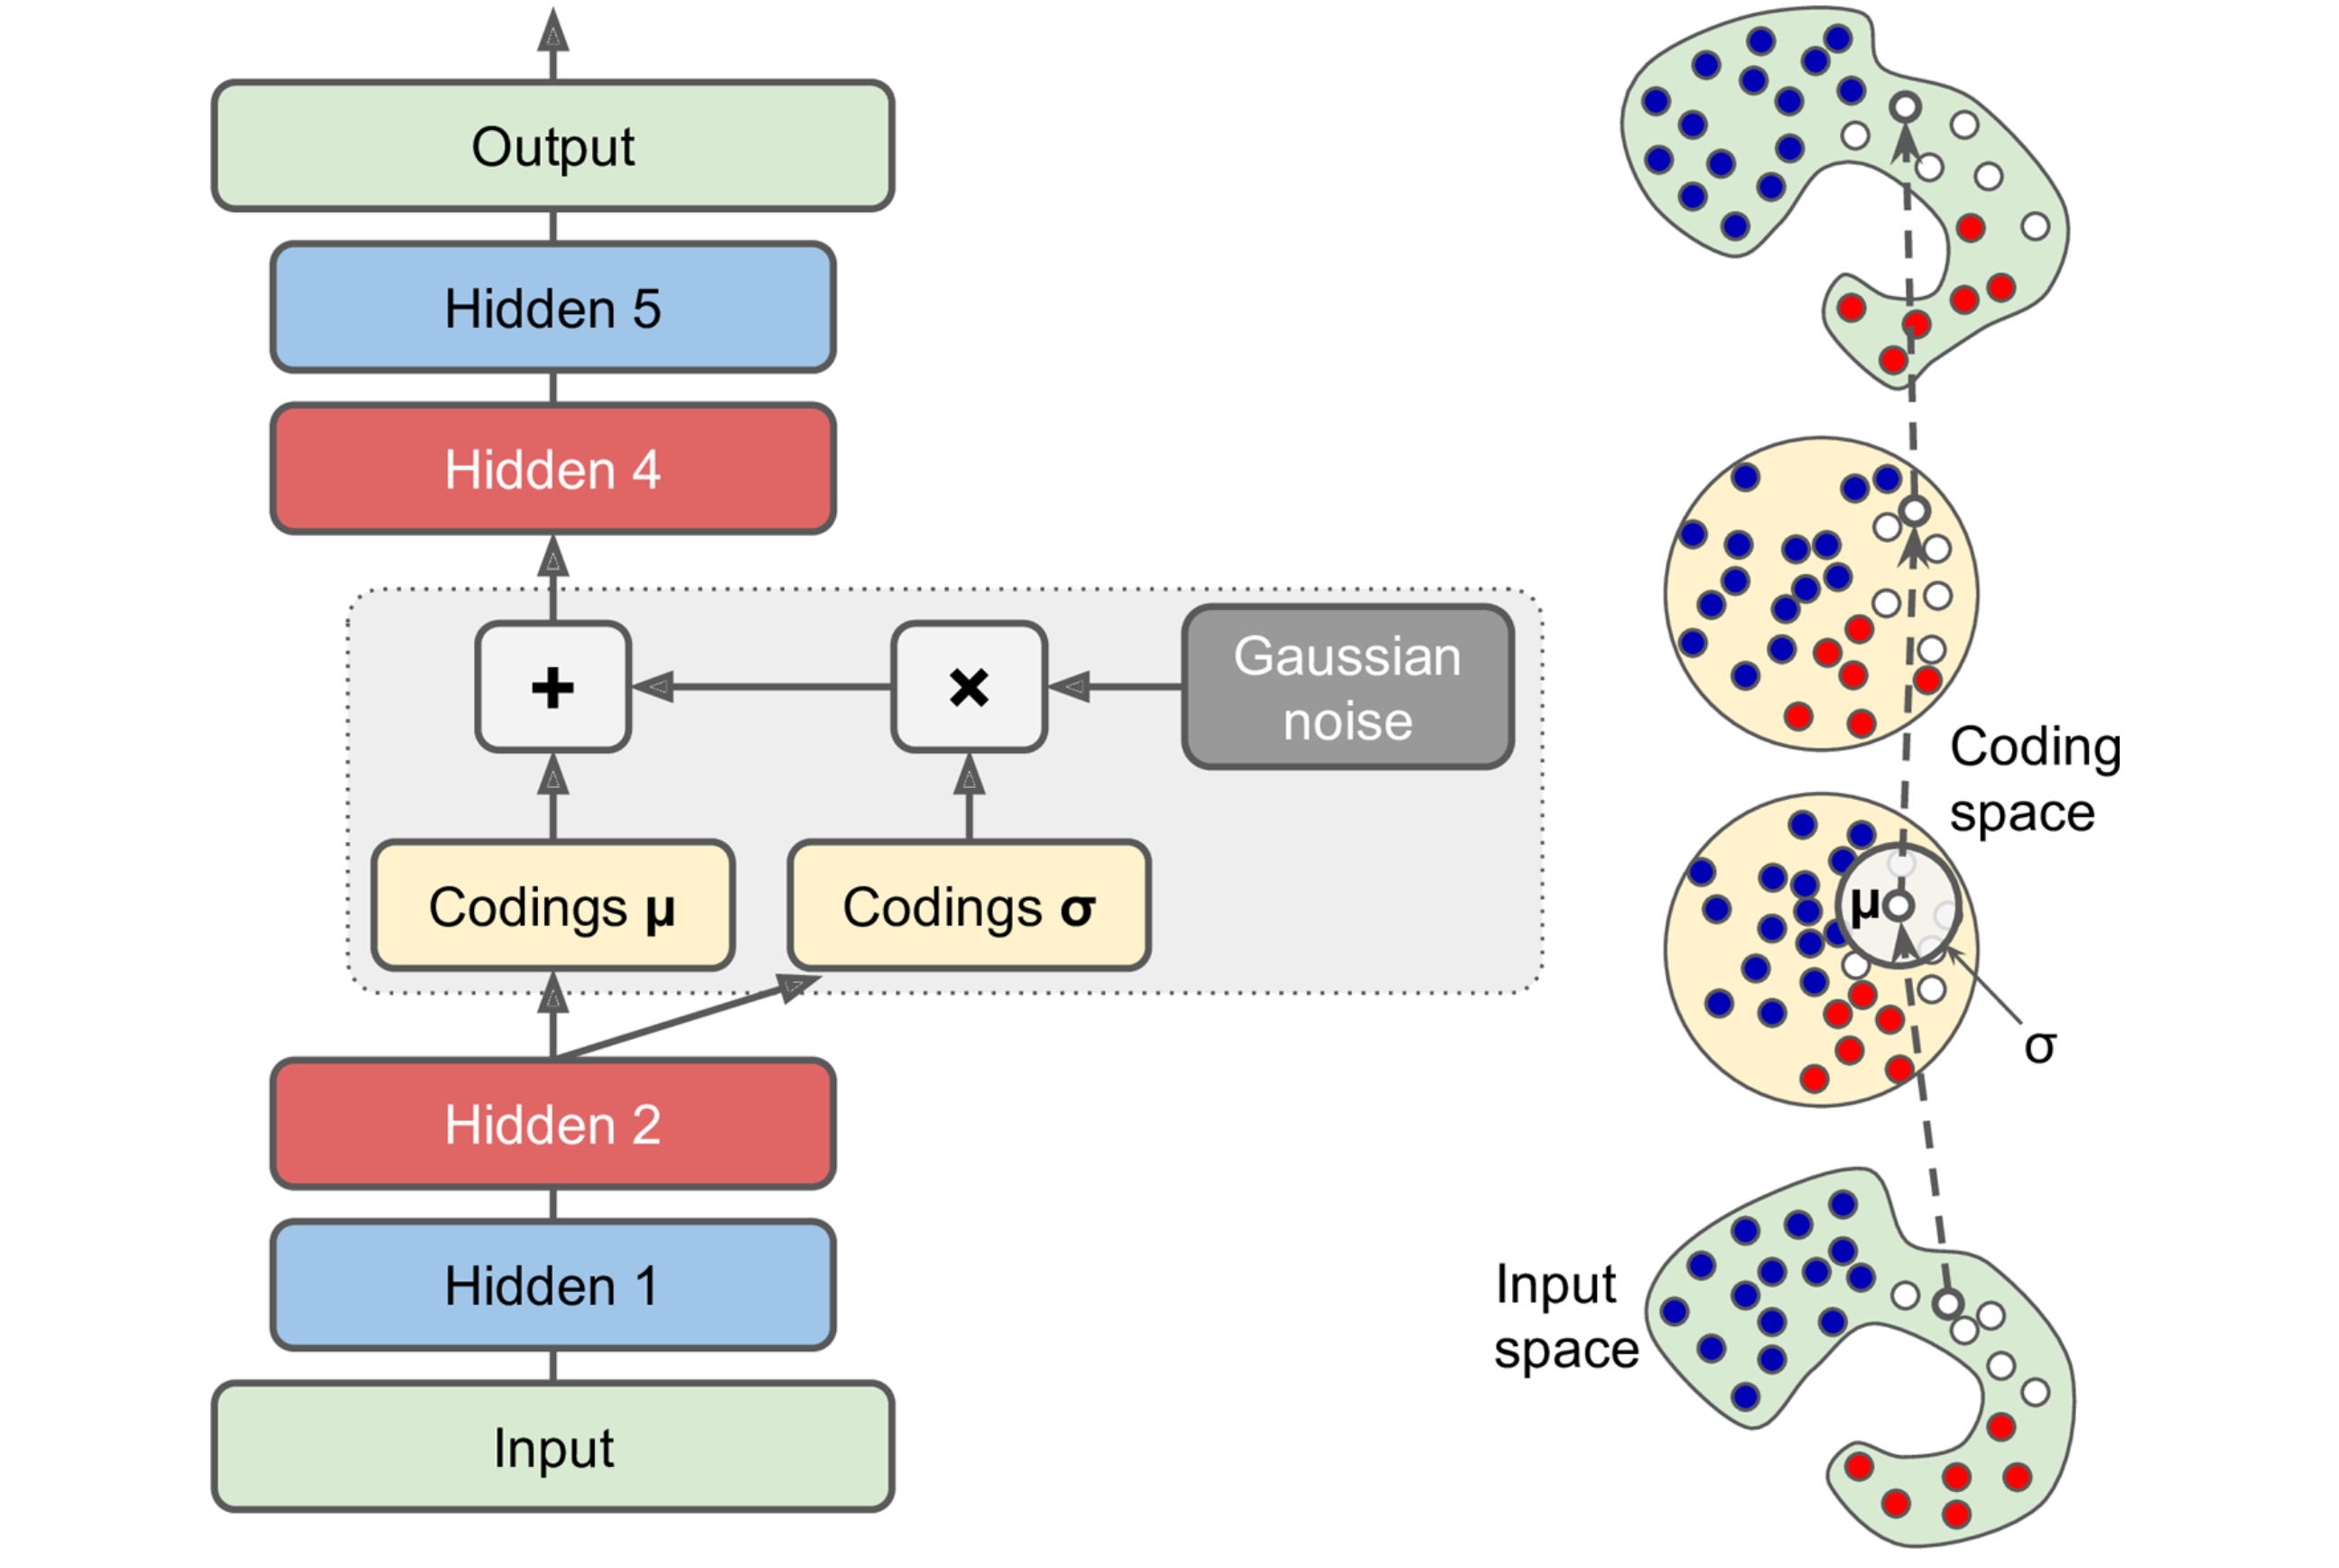
\includegraphics[width=8cm]{vae_arch}
    \end{figure}}

\end{itemize}
}

%%%%%%%%%%%%%%%%%%%%%%%%%%%%%%%%%%%%%%%%%%%%%%%%%%%%%%%%%%%%%%%%%%%%%%%%%%%%%%%%%%%%%%%%%%%%%%%

\frame{\frametitle{Variational Autoencoders}

    
    \begin{figure}[htp]
    \centering
    \hyperlink{vae}{
    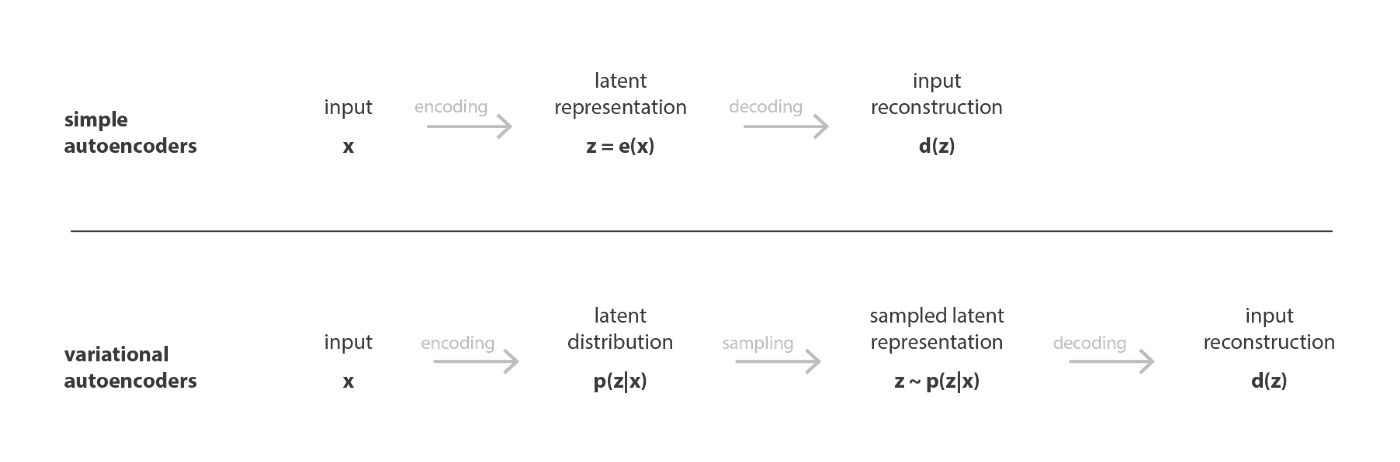
\includegraphics[width=9cm]{vae_6}}

    \vspace{1 pt}
    
    \hyperlink{vae}{
    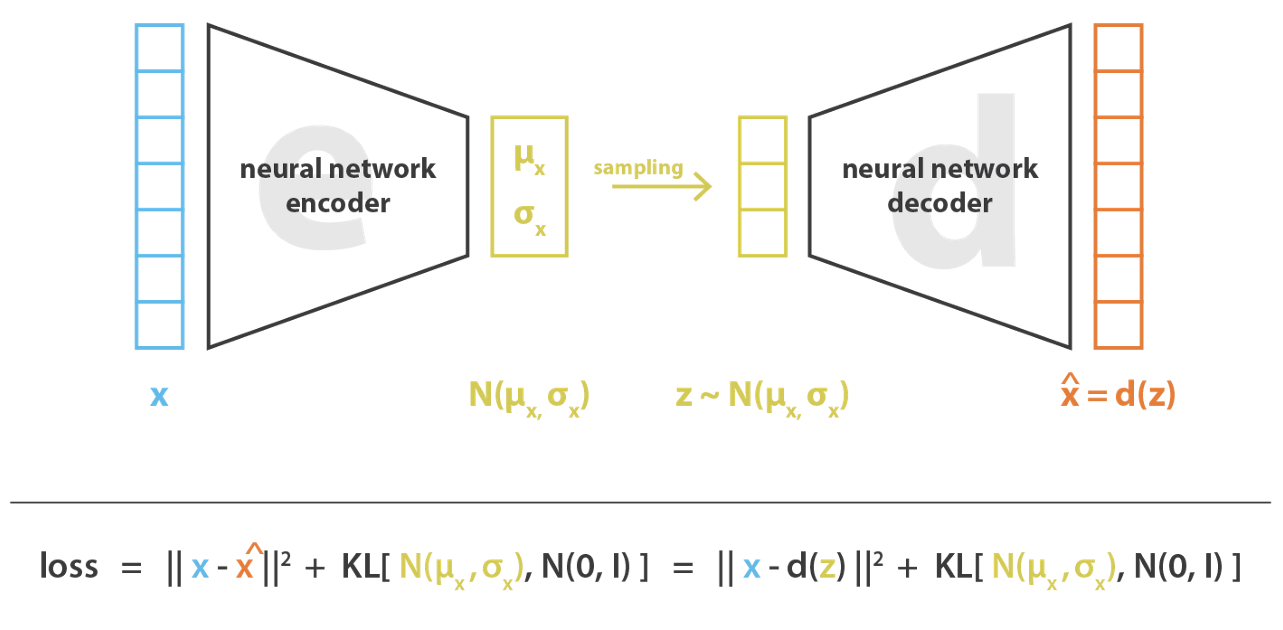
\includegraphics[width=9cm]{vae_4_1}}
    \end{figure}

}

%%%%%%%%%%%%%%%%%%%%%%%%%%%%%%%%%%%%%%%%%%%%%%%%%%%%%%%%%%%%%%%%%%%%%%%%%%%%%%%%%%%%%%%%%%%%%%%

\frame{\frametitle{Test}
	
	
\begin{itemize}
	\item One
	\begin{itemize}
		\item One
		\item Two
		\item Three
	\end{itemize}

	\item 
	For two-dimensional tensors, we have a corresponding sum with indices $(a, b)$ for $f$ and $(i-a, j-b)$ for $g$, respectively:
	$$
	(f * g)(i, j)=\sum_a \sum_b f(a, b) g(i-a, j-b)
	$$
	
	\item 
	
	It is given by,
	$$
	\left.w_{t+1}=w_t-\left(\alpha_t / \sqrt{\left(v_t\right.}\right)+e\right) *\left(\delta L / \delta w_t\right)
	$$
	where,
	$$
	v_t=\beta * v_t+(1-\beta) *\left(\delta L / \delta w_t\right)^2
	$$
\end{itemize}	
	
}

%%%%%%%%%%%%%%%%%%%%%%%%%%%%%%%%%%%%%%%%%%%%%%%%%%%%%%%%%%%%%%%%%%%%%%%%%%%%%%%%%%%%%%%%%%%%%%%
\frame{\frametitle{Image References}
	
\begin{itemize}
    
    \item
    \hypertarget{ae_arch}{https://lilianweng.github.io/posts/2018-08-12-vae/}
    
    \item
    \hypertarget{bad_ae}{https://emkademy.medium.com/1-first-step-to-generative-deep-learning-with-autoencoders-22bd41e56d18}
    
    \item
    \hypertarget{AE}{Aurelien Geron. 2019. Hands-On Machine Learning with Scikit-Learn, Keras, and TensorFlow: Concepts, Tools, and Techniques to Build Intelligent Systems (2nd. ed.). O'Reilly Media, Inc.}
    
    \item
    \hypertarget{generated_by_VAE}{https://github.com/wojciechmo/vae}
    
	\item 
	\hypertarget{watermark_removal}{https://ai.googleblog.com/2017/08/making-visible-watermarks-more-effective.html}
	
	\item
	\hypertarget{noise_reduction}{https://medium.com/@harishr2301/denoising-autoencoders-996e866e5cd0}
	
	\item 
	\hypertarget{stacked_ae}{
	https://subscription.packtpub.com/book/big-data-and-business-intelligence/9781787121089/4/ch04lvl1sec51/setting-up-stacked-autoencoders}
	
	\item
	\hypertarget{ae_1}{https://www.analyticsvidhya.com/blog/2021/01/auto-encoders-for-computer-vision-an-endless-world-of-possibilities/}
	
	\item
	\hypertarget{cnn_ae}{https://towardsdatascience.com/convolutional-autoencoders-for-image-noise-reduction-32fce9fc1763}
	
	\item
	\hypertarget{denoising}{https://ift6266h17.files.wordpress.com/2017/03/14\_autoencoders.pdf}
	
	\item
	\hypertarget{vae}{https://towardsdatascience.com/understanding-variational-autoencoders-vaes-f70510919f73}


	
	
\end{itemize}	
}

%%%%%%%%%%%%%%%%%%%%%%%%%%%%%%%%%%%%%%%%%%%%%%%%%%%%%%%%%%%%%%%%%%%%%%%%%%%%%%%%%%%%%%%%%%%%%%%

\frame{\frametitle{References}
	
\begin{itemize}
    
    \item
    Aurelien Geron. 2019. Hands-On Machine Learning with Scikit-Learn, Keras, and TensorFlow: Concepts, Tools, and Techniques to Build Intelligent Systems (2nd. ed.). O'Reilly Media, Inc.
    
    \item
    https://www.cs.toronto.edu/~rgrosse/courses/csc321\_2017/slides/lec20.pdf
    
    \item
    https://www.math.purdue.edu/~buzzard/MA598-Spring2019/Lectures/Lec16\%20-\%20Autoencoders.pptx
    
    \item
    http://cs231n.stanford.edu/slides/2019/cs231n\_2019\_lecture11.pdf
    
	
\end{itemize}	
}

%%%%%%%%%%%%%%%%%%%%%%%%%%%%%%%%%%%%%%%%%%%%%%%%%%%%%%%%%%%%%%%%%%%%%%%%%%%%%%%%%%%%%%%%%%%%%%%

\frametitle{Final Notes}
\centering
\vspace{50 pt}
\textbf{Thank You!}
\vspace{50pt}

\textbf{Any Question?}
%%%%%%%%%%%%%%%%%%%%%%%%%%%%%%%%%%%%%%%%%%
\end{document}